\documentclass[page number]{beamer}
\usepackage{etex}
\usepackage{graphicx, booktabs} % For tabulars
\usepackage{pgf,tikz}
\usepackage{ulem}
\usetikzlibrary{arrows}
\usetikzlibrary{positioning,shapes,fit}
\usepackage{algorithm}
\usepackage{algpseudocode}
\usepackage{multicol}
\usepackage{syntax}
\usepackage{xcolor, color, colortbl}
\usepackage{tikz-qtree}
\usepackage{listings}

\input{style}

\makeatletter
\input{cmds}
\makeatother

\setcounter{tocdepth}{1} % remove subsection from table of contents

%counting frames
\newcommand{\backupbegin}{
   \newcounter{framenumberappendix}
   \setcounter{framenumberappendix}{\value{framenumber}}
}
\newcommand{\backupend}{
   \addtocounter{framenumberappendix}{-\value{framenumber}}
   \addtocounter{framenumber}{\value{framenumberappendix}}
}


\begin{document}
\title[Int-Ptr casts in CompCert]{Implementing a memory model supporting int-ptr casts in CompCert}


\author{Aur\`ele Barri\`ere}

\def\todo#1{{\color{red}TODO:\quad#1}}
\def\addref#1{{\color{red}$[$#1$]$}}
\def\undef{\textit{undef}}
\def\states#1{\mathit{States_{#1}}}
\def\step#1{\mathit{Step_{#1}}}
\def\atstep#1{\mathit{AtomicStep_{#1}}}
\def\traces{\mathit{Traces}}
\def\comment#1{{\color{blue}\textit{#1}}}
\def\outline{
  \begin{frame}
    \frametitle{Outline}
    \tableofcontents[currentsection]
  \end{frame}
}


\lstset{%
  basicstyle=\footnotesize,
  language=C,
  keywordstyle=\color{basicPurple}\textbf,
  float
}

\begin{frame}[plain]
  \titlepage%
  \vfill
  \begin{center}
    \includegraphics[width=2.5cm]{img/enslogo.png}
    \hfill
    \includegraphics[width=2.5cm]{img/snulogo.png}
  \end{center}
\end{frame}

\section{Introduction}
\begin{frame}{\secname : Integer-Pointer casting in C}

  \comment{Example}
  \vfill
  \begin{alertblock}{ISO C Standard}
  \end{alertblock}
  \vfill
  \begin{exampleblock}{Uses}
  \end{exampleblock}
  
\end{frame}

\begin{frame}{Giving semantics to Integer-Pointer Casts in C}

  \comment{A new memory model with semantics and optimizations}\\
  \comment{Reference the paper}\\
  \comment{The benefits of giving semantics to cast}
  
\end{frame}


\begin{frame}{CompCert: a certified C compiler}

  \begin{block}{CompCert}
    \begin{itemize}
      \item From C to ASM (x86, powerpc or arm).
      \item Most passes are proved in Coq.
      \item Supports most of the ISO-C-99 standard.
    \end{itemize}
  \end{block}
  \vfill
  \begin{center}
    \includegraphics[scale=0.6]{img/passes.png}
  \end{center}
  
\end{frame}


\begin{frame}{Aim of this work}
  
  \begin{block}{Goals}
    \begin{itemize}
    \item Implement the new memory model in CompCert.
    \item Prove the correctness of compilation with this new model.
    \end{itemize}
  \end{block}
  \vfill
  \begin{exampleblock}{Benefits}
    \begin{itemize}
    \item Relevance and usability of the new memory model and semantics.
    \item Allow CompCert to compile correctly a bigger set of C programs.
    \end{itemize}
  \end{exampleblock}

\end{frame}


\section{C Memory Models}
\outline
\subsection{Logical Memory Model}
\begin{frame}{\subsecname}

  \begin{block}{Memory blocks}
    $$\texttt{Block}=\{(v,n,c)~|~v\in\texttt{Bool},n\in\mathbb{N},c\in\texttt{Val}^{n}\}$$
  \end{block}
  \vfill
  \comment{Optimization examples}
  \vfill
  \begin{alertblock}{No semantics for Integer-Pointer cast}
    \comment{A few things are still defined}
  \end{alertblock}
  
\end{frame}

\subsection{Concrete Memory Model}
\begin{frame}{\subsecname}

  \begin{block}{Memory blocks}
    $$\texttt{Block}=\{(p,n)~|~p\in\texttt{int32},n\in\texttt{int32}\}$$
  \end{block}
  \vfill
  \begin{block}{Memory Consistency}
    \begin{itemize}
    \item \textbf{No overflow:} $\quad\forall (p,n)\in\texttt{Allocated}, [p,p+n]\subseteq]0,2^{32}[$.
      \item \textbf{No overlap:} $\quad\forall (p_1,n_1), (p_2,n_2)\in\texttt{Allocated},$\\ $[p_1,p_1+n_1]\text{ and }[p_2,p_2+n_2]\text{ are disjoint.}$
    \end{itemize}
  \end{block}
  \vfill
  \begin{alertblock}{No optimizations}
    No ownership of memory blocks.
  \end{alertblock}

\end{frame}

\subsection{Quasi-Concrete Memory Model}
\begin{frame}{\subsecname}

  \begin{block}{Memory blocks}
    \begin{itemize}
    \item $\texttt{Block}=\{(v,p,n,c)~|~v\in\texttt{Bool},n\in\mathbb{N},c\in\texttt{Val}^{n},p\in\texttt{int32}\cup\{\undef\}\}$.
    \item Memory consistency (\textbf{No overflow}, \textbf{No overlap}) for concrete blocks.
    \end{itemize}
  \end{block}
  \vfill
  \begin{exampleblock}{Properties}
    \begin{itemize}
    \item Optimizations are possible with logical blocks.
    \item Integer-Pointer cast is posible with concrete blocks.
    \end{itemize}
  \end{exampleblock}
  
\end{frame}

\begin{frame}{The Capture Function}

  \comment{Capture before every cast}\\
  \comment{examples of optimizations}
  \vfill
  \begin{alertblock}{Non-determinism}
    A logical block can be captured at several different addresses.
  \end{alertblock}
  
\end{frame}


\section{Contribution}
\outline
\def\backward{
  \begin{figure}
    \centering
    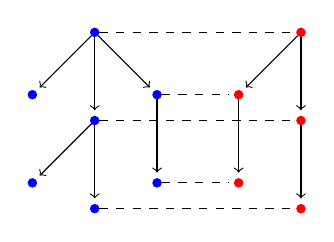
\begin{tikzpicture}[%
        every node/.style={circle,minimum size=3pt,minimum height=3pt, inner sep=0pt},
        shorten >=2pt,
        node distance=1cm
      ]
      \node [draw] (0) [color=blue, fill] {};
      \node [draw] (1) [color=blue, fill, below left=of 0] {};
      \node [draw] (2) [color=blue, fill, below=of 0] {};
      \node [draw] (3) [color=blue, fill, below right=of 0] {};
      \node [draw] (4) [color=blue, fill, below left=of 2] {};
      \node [draw] (5) [color=blue, fill, below=of 2] {};
      \node [draw] (6) [color=blue, fill, below=of 3] {};
      \node [draw] (7) [color=red, fill, right=of 0, xshift=1.5cm] {};
      \node [draw] (8) [color=red, fill, below left=of 7] {};
      \node [draw] (9) [color=red, fill, below=of 7] {};
      \node [draw] (10) [color=red, fill, below=of 8] {};
      \node [draw] (11) [color=red, fill, below=of 9] {};
      \path [draw] (0) edge[->]  node {} (1)
      (0) edge[->]  node {} (2)
      (0) edge[->]  node {} (3)
      (2) edge[->]  node {} (4)
      (2) edge[->]  node {} (5)
      (3) edge[->]  node {} (6)
      (7) edge[->]  node {} (8)
      (7) edge[->]  node {} (9)
      (8) edge[->]  node {} (10)
      (9) edge[->]  node {} (11);
      \draw[dashed] (0) -- (7);
      \draw[dashed] (3) -- (8);
      \draw[dashed] (2) -- (9);
      \draw[dashed] (5) -- (11);
      \draw[dashed] (6) -- (10);
    \end{tikzpicture}
    \label{fig:backward}
  \end{figure}
}

\def\forward{
  \begin{figure}
    \centering
    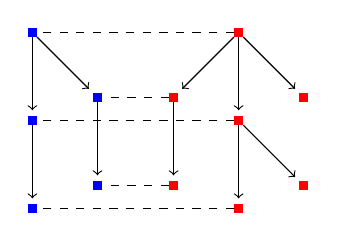
\begin{tikzpicture}[%
        every node/.style={rectangle,minimum size=3pt,minimum height=3pt, inner sep=0pt},
        shorten >=2pt,
        node distance=1cm
      ]
      \node [draw] (0) [color=red, fill] {};
      \node [draw] (1) [color=red, fill, below right=of 0] {};
      \node [draw] (2) [color=red, fill, below=of 0] {};
      \node [draw] (3) [color=red, fill, below left=of 0] {};
      \node [draw] (4) [color=red, fill, below right=of 2] {};
      \node [draw] (5) [color=red, fill, below=of 2] {};
      \node [draw] (6) [color=red, fill, below=of 3] {};
      \node [draw] (7) [color=blue, fill, left=of 0, xshift=-1.5cm] {};
      \node [draw] (8) [color=blue, fill, below right=of 7] {};
      \node [draw] (9) [color=blue, fill, below=of 7] {};
      \node [draw] (10) [color=blue, fill, below=of 8] {};
      \node [draw] (11) [color=blue, fill, below=of 9] {};
      \path [draw] (0) edge[->]  node {} (1)
      (0) edge[->]  node {} (2)
      (0) edge[->]  node {} (3)
      (2) edge[->]  node {} (4)
      (2) edge[->]  node {} (5)
      (3) edge[->]  node {} (6)
      (7) edge[->]  node {} (8)
      (7) edge[->]  node {} (9)
      (8) edge[->]  node {} (10)
      (9) edge[->]  node {} (11);
      \draw[dashed] (0) -- (7);
      \draw[dashed] (3) -- (8);
      \draw[dashed] (2) -- (9);
      \draw[dashed] (5) -- (11);
      \draw[dashed] (6) -- (10);
    \end{tikzpicture}
    \label{fig:forward}
  \end{figure}
}

\def\mixed{
  \begin{figure}
    \centering
    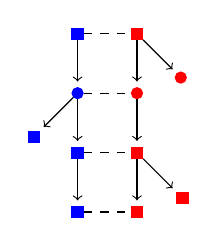
\begin{tikzpicture}[%
        every node/.style={rectangle,minimum size=4pt,minimum height=4pt, inner sep=0pt},
        shorten >=2pt,
        node distance=0.6cm
      ]
      \node [draw] (0) [color=blue, fill] {};
      \node [draw] (1) [circle, color=blue, fill, below=of 0] {};
      \node [draw] (2) [color=blue, fill, below left=of 1] {};
      \node [draw] (3) [color=blue, fill, below=of 1] {};
      \node [draw] (4) [color=blue, fill, below=of 3] {};
      \node [draw] (5) [color=red, fill, right=of 0] {};
      \node [draw] (6) [circle, color=red, fill, below=of 5] {};
      \node [draw] (7) [circle, color=red, fill, below right=of 5] {};
      \node [draw] (8) [color=red, fill, below=of 6] {};
      \node [draw] (9) [color=red, fill, below=of 8] {};
      \node [draw] (10) [color=red, fill, below right=of 8] {};
      \path [draw] (0) edge[->]  node {} (1)
      (1) edge[->]  node {} (2)
      (1) edge[->]  node {} (3)
      (3) edge[->]  node {} (4)
      (5) edge[->]  node {} (6)
      (5) edge[->]  node {} (7)
      (6) edge[->]  node {} (8)
      (8) edge[->]  node {} (9)
      (8) edge[->]  node {} (10);
      \draw[dashed] (0) -- (5);
      \draw[dashed] (1) -- (6);
      \draw[dashed] (3) -- (8);
      \draw[dashed] (4) -- (9);
    \end{tikzpicture}
    \label{fig:mixed}
  \end{figure}
}

\subsection{Memory Update}
\begin{frame}{\subsecname}

  \begin{block}{Updating the definition of the memory}
    \begin{itemize}
    \item Add a map \texttt{mem\_concrete: block -> Option Z}.
    \item Remember the size of blocks at allocation.
    \item Address-wise permissions.
    \end{itemize}
  \end{block}
  \vfill
  \begin{block}{Abstract Analysis}
    The stack block can be accessible if it is concrete.
  \end{block}
    \vfill
    \begin{exampleblock}{Proofs}
      \begin{itemize}
      \item Every memory operation preserves memory consistency.
      \item Abstract analysis is sound.
      \end{itemize}
  \end{exampleblock}

  
\end{frame}

\subsection{Memory Injection}
\begin{frame}{\subsecname}

  \begin{block}{Memory Injection}
    A map from some blocks of the source memory to blocks of the target memory.
  \end{block}
  \vfill
  \begin{block}{Changes}
  Concrete blocks in the source should be preserved, at the same address, in the target.
  \end{block}
  \vfill
  \begin{exampleblock}{Proofs}
    Every memory operation preserves memory injection.
  \end{exampleblock}
  
\end{frame}

\subsection{Capture Insertion}
\begin{frame}{\subsecname}

  \begin{block}{Insert capture before each cast}
  Done by Juneyoung Lee.\\
  Between CompCert C and Clight.
  \end{block}
  \vfill
  \begin{tabular}{l c r}        
    \lstinputlisting[linewidth=4cm]{listings/captureinsert.c} &
    $\longrightarrow$ & 
    \lstinputlisting[linewidth=6.2cm]{listings/captureinsert.clight}
  \end{tabular}

\end{frame}

\subsection{Mixed Simulations}
\begin{frame}{Proving the correctness of CompCert}
  \begin{columns}[T] % align columns
    \begin{column}{.48\textwidth}
      \begin{block}{Backward Simulation}
        Step in target $\rightarrow$\\ Matching step in source\\
        {\color{blue}Source\hfill\color{red}Target}
        \backward
      \end{block}
    \end{column}%
    \hfill
    \begin{column}{.48\textwidth}
      \begin{block}{Forward Simulation}
        Step in source $\rightarrow$\\ Matching step in target\\
        {\color{blue}Source\hfill\color{red}Target}
        \forward
      \end{block}
    \end{column}%
  \end{columns}
\end{frame}

\begin{frame}{Changing the correctness proof}
  \begin{exampleblock}{Goal}
    A backward simulation between C and ASM.
  \end{exampleblock}
  \vfill
  \begin{alertblock}{Previous proof}
    Determinacy + forward simulation $\rightarrow$ backward simulation.\\
    No more determinacy!
  \end{alertblock}
  \vfill
  \begin{exampleblock}{Handling non-deterministic behavior}
    Non-deterministic behavior only for the capture function.\\
    For every other state, we still have local determinacy.
  \end{exampleblock}
\end{frame}

\begin{frame}{Mixed Simulations}
  \begin{block}{Mixed Simulation}
    External state ($\bigcirc$): Local backward simulation.\\
    Internal state ($\Box$): Local forward simulation.\\
    {\color{blue}Source\hfill\color{red}Target}
    \vspace{-0.8cm}
    \mixed
  \end{block}
  \vfill
  \begin{block}{Theorem}
    MixedSim (A,B) $\rightarrow$ BackwardSim ((atomic A),B).
  \end{block}
\end{frame}

%\begin{frame}{The previous correctness proof}
%  \oldprooffwds
%  \vfill
%  \begin{block}{Theorem}
%    Forward Simulation Composition.
%  \end{block}
%\end{frame}
%
%\begin{frame}{The previous correctness proof}
%  \oldprooffwd
%  \vfill
%  \begin{block}{Theorems}
%  \begin{itemize}
%    \item ForwardSim(A,B) $\rightarrow$ BackwardSim(atomic(A),B).
%    \item BackwardSim(A,B) $\rightarrow$ BackwardSim(A,atomic(B)).
%  \end{itemize}
%  \end{block}
%\end{frame}
%
%\begin{frame}{The previous correctness proof}
%  \oldprooffactorbwd
%  \vfill
%  \begin{block}{Theorem}
%    Backward Simulation Composition.
%  \end{block}
%\end{frame}
%
%\begin{frame}{The previous correctness proof}
%  \oldprooffinal
%\end{frame}
%
\begin{frame}{The new correctness proof}
  \proofmixed
  \vfill
  \begin{block}{Theorem}
    MixedSim (A,B) $\rightarrow$ BackwardSim ((atomic A),B).
  \end{block}
\end{frame}

\begin{frame}[noframenumbering]{The new correctness proof}
  \proofmixedbwd
  \vfill
  \begin{block}{Theorem}
    BackwardSim(A,B) $\rightarrow$ BackwardSim(A,atomic(B)).
  \end{block}
\end{frame}

\begin{frame}[noframenumbering]{The new correctness proof}
  \proofatbwd
  \vfill
  \begin{block}{Theorem}
    Backward Simulation Composition.
  \end{block}
\end{frame}

\begin{frame}[noframenumbering]{The new correctness proof}
  \prooffinal
\end{frame}



\section{Evaluation}
\outline
\begin{frame}{\secname: Correctness}

  \begin{alertblock}{Admitted Theorems}
    Most mixed simulations.
  \end{alertblock}
  \vfill
  \begin{exampleblock}{Finishing the proofs}
    Two mixed simulations finished. Others should be very similar.
  \end{exampleblock}
  \vfill
  \begin{alertblock}{Casts semantics not fully implemented}
    We can still see the capture, and compile some C programs.
  \end{alertblock}
  
\end{frame}

\begin{frame}{\secname: Optimizations}
  \begin{tabular}{l c r}
    \lstinputlisting[linewidth=4cm]{listings/evallogical.c} &
    $\longrightarrow$ &
    \lstinputlisting[linewidth=6cm]{listings/evallogicalopt.c}
  \end{tabular}
  \vfill
  \hrulefill
  \vfill
  \begin{tabular}{l c r}
    \lstinputlisting[linewidth=4cm]{listings/evalconcrete.c} &
    $\longrightarrow$ & 
    \lstinputlisting[linewidth=6.5cm]{listings/evalconcreteopt.c}
  \end{tabular}

\end{frame}


\section{Conclusion}
\begin{frame}{\secname}

  \begin{exampleblock}{Results}
    \begin{itemize}
    \item The new memory model has been implemented in CompCert.
    \item It successfully gives semantics to Integer-Pointer casts.
    \item It allows optimizations.
    \item The proof of correctness is almost finished.
    \item Already added 5kloc of Coq.
    \end{itemize}
  \end{exampleblock}
  \vfill
  \begin{block}{Future Work}
    \begin{itemize}
    \item Finish the mixed simulations proofs.
    \item Finish implementation of the integer-pointer cast semantics.
    \end{itemize}
  \end{block}
  
\end{frame}


\end{document}
